\documentclass[a4paper, 12pt]{article}

\usepackage[english]{babel}
\usepackage[utf8x]{inputenc}
\usepackage{amsmath}
\usepackage{graphicx}
\usepackage{csquotes}
\usepackage[hidelinks]{hyperref}
\usepackage{booktabs}
\usepackage{listings}
\usepackage[style=mla]{biblatex}

\usepackage{colortbl}% http://ctan.org/pkg/colortbl
\usepackage{xcolor}% http://ctan.org/pkg/xcolor

\newcounter{examplecounter}
\newenvironment{example}{\begin{quote}%
    \refstepcounter{examplecounter}%
  \textbf{Example \arabic{examplecounter}}%
  \quad
}{%
\end{quote}%
}

\newcommand{\ra}[1]{\renewcommand{\arraystretch}{#1}}
\colorlet{tableheadcolor}{gray!25} % Table header colour = 25% gray
\newcommand{\headcol}{\rowcolor{tableheadcolor}} %
\colorlet{tablerowcolor}{gray!10} % Table row separator colour = 10% gray
\newcommand{\rowcol}{\rowcolor{tablerowcolor}} %

\title{Shadow Volumes using Geometry Shader}
\author{Nora Björklund \and Johan Jönsson}

\begin{document}
\maketitle
\tableofcontents
\newpage
\section{Introduction}
Shadow Volumes is a common way of creating real-time hard-shadows, and has been used in games such as Doom 3 \footcite{gpug1}. In this project, the shadow volumes are implemented with the geometry shader. Implementation by geometry shader takes tedious vertex related processing away from the CPU, and insted uses the simultaneous processing power of the GPU.[REF]
\subsection{Project Goal}
The following goals was setup before the start of the project:
\begin{itemize}
\item Implement shadow volumes
\item Place different object in the ``world''
\item Place light-sources
\item Compare to a pre-generated scene 
\item Soft Shadows
\end{itemize}
If we have time over we wanted to implement the following tasks:
\begin{itemize}
\item Material med olika optiska egenskaper (transparens, brytningsindex)
\item  ”Fancy” GUI
\item  Different levels of difficulty (exactness of the shadows compared to the pregenerated)
\item  Reflective surfaces (why make it simple)
\item  Score board (since it is a game)
\item  Time limitations (stress is fun)
\item  Comparision with Shadow Maps (another game version?)
\item  Leap Motion-control (seems cool!)
\end{itemize}

Due to sevaral problems that occured when implementing the shadow volumes, the project has been compromised to shadow volumes created with the help of the geometry shader and erroneus shadows. There are controls implemented to move around in the small world and simple controls to show/hide the shadow volumes, and move one of the bunny-objects that exists in the world. However, no game element has been implemented. It is still a fun game idea to continue working on further.
\section{Background}
In this section short backgrounds to the techniques used in this project are given.
\subsection{Shadow Volumes}
The shadow volume algorithm was first proposed in 1977 by computer scientist Franklin Crow \footcite{CROW77}. Later in 1991, Tim Heidmann published a paper describing the sillhouette detection by using the stecil buffer based on the shadow volumes \footcite{HEIDMANN91}. Using the stencil buffer for silhouette detection is still today the main algorith for shadows with shadow volumes \footcite{KOLIVAND13}. 

The method Heidmann described is more commonly called the Z-pass or Depth Pass, and is also the one which we implemented in this project. Another algorithm is the Z-fail/Depth Fail, which deals with the problem that occurs in Z-pass when the observer/camera is inside the shadow volume. 
\subsection{Geometry Shader}
The Geometry shader has been a core part of OpenGL since version 3.2 \footcite{GEOM}. It is placed between the Vertex shader and the Vertex post-processing stages (such as primitive assembly and rasterization), and takes care of processing of primitives. It can recieve one single primitive and output a set of primitives (an output of no primitives is also possible).

A geometry shader is defined to take a specific type of primitive where the available types are defined in table \ref{tab:GSprimitives}.

\begin{table}
\centering
\caption{Table showing the types of input and output primitives that a geometry shader can process, from \footcite{GEOM}. Here the vertex count is the number of vertices that geometry shaders recieves for every input primitive }
\label{tab:GSprimitives}
\begin{tabular}{lll} \toprule
GS Input & OpenGL primitives & Vertex Count \\\headcol \midrule
\headcol points& GL\_POINTS​&1\\
\rowcol lines& GL\_LINES​, GL\_LINE\_STRIP​​&2\\
\rowcol &  GL\_LINE\_LIST&\\
\headcol lines\_adjacency&GL\_LINES\_ADJACENCY​&​3\\
\headcol & GL\_LINE\_STRIP\_ADJACENCY&\\
\rowcol triangles&GL\_TRIANGLES​​&4\\
\rowcol & GL\_TRIANGLE\_STRIP​&\\
\rowcol &GL\_TRIANGLE\_FAN&\\
\headcol triangles\_adjacency&GL\_TRIANGLES\_ADJACENCY​​&6\\
\headcol & GL\_TRIANGLE\_STRIP\_ADJACENCY&\\\midrule
\end{tabular}
\end{table}

The allowed output primitives are \emph{points}, \emph{line\_strip}, \emph{triangle\_strip}.

In a geometry shader program, the input and outputs are defined in the beginning of the geometry shader program, before the main-loop, as follows;
\begin{center}
\textbf{layout(input\_primitive​) in;}
\end{center}
Where the input primitive can be any of the ones given in table \ref{tab:GSprimitives}. 
\begin{center}
\textbf{layout(output\_primitive​, max\_vertices = vert\_count​) out;}
\end{center}
Here the max\_vertices must be defined, and is the maximum number of vertices that can be emitted in one pass through the shader.

A pass-through geometry shader looks like the one in example \ref{ex:pass_through}. It is useless in itself but allows us a quick look at the simplest syntax of the shader. 
\newpage 
\begin{example}\label{ex:pass_through}
\hrule
\begin{lstlisting}[language=c]
#version 150 
layout(triangles_adjacency) in;
layout(triangle_strip, max_vertices=3) out;
in vec3 ex_Position[];
in vec3 ex_Normal[];
in vec2 ex_TexCoord[];
out vec3 f_Normal;
out vec2 f_TexCoord;	     
out vec3 f_Position;

void main()
{
   //For pass through
   for(int i = 0; i < gl_in.length(); i += 2)
    {
       // copy attributes
      gl_Position = gl_in[i].gl_Position;
      f_Normal = ex_Normal[i];
      f_TexCoord = ex_TexCoord[i]; 
      f_Position = ex_Position[i];
 
      // done with the vertex
       EmitVertex();
    }
   EndPrimitive();
}
\end{lstlisting}
\hrule
\end{example}

\section{Implementation}
In this chapter we will describe how we implemented the different parts of the project. We begin by discussing the overall structure of the program and then we dive into detail on the object loader and how we generate the shadow volumes using the geometry shader.
\subsection{Program Structure}
In figure XX an outline of the program structure can be seen. In the main file we can, as in most computer graphic programs we have used in TSBK07 and TSBK03, see that we have a main loop that is using the two functions \textbf{init} and \textbf{display}. We have also added functions for orientation by mouse-movements (\textbf{mouse\_passive\_move}), movements and other functions implemented with keyboard clicks (\textbf{keyboard}), picking up/setting down objects (\textbf{MouseClickFunc}). 

In the init function all the initial values and settings are set-up. Here we initiate the World, a class holding all the objects in the program. The objects can for example be point objects such as the camera or the light-source,  or visual objects like bunnies and ground/grass.

These objects are then controlled and updated in the display loop. It is also here that we implement the shadow volume algorithm. All the objects in the world have the attributes position and rotation, and functions for placing them in other parts of the world, translation, rotation. The object class is then divided into subclasses further defining their individual properties.  

We have implemented a z-pass version of the shadow volumes algorithm. We begin
by turning off the colour buffer rendering the scene into the depth buffer and
writing zeros into the stencil buffer (using GL\_NEVER, 0 and G\_REPLACE on
stencil fail). Next we turn off writing to the depth buffer, turn on back face
culling, render the scene and increase the stencil buffer on z-pass. Then we
turn on front face culling and decrement the stencil buffer on z-pass. This way
any part of the scene in shadows will have a non-zero value in the stencil
buffer, we turn the color buffer back on and render all lit parts of the scene
using the stencil buffer (without changing the values in the stencil buffer).
Finally we disable the stencil buffer and turn depth testing back on.

\subsection{Object Loader}
In order to produce proper shadow volumes it is necessary to know the neighbours
of each vertex. Passing this information to the shader is a simple process since
OpenGL has built in support for adjacency primitives. All we need to do is
extract the adjacency information for each object, before we upload them to the
shader. This introduces the need for an object loader capable of extracting this
information at the time of loading the objects in the initialization step.

In order to achieve this it was necessary to write a new object loader, more or
less from scratch (inspiration was of course taken from the functions in
loadobj.~c). For this new object loader we decided to use the open source library
assimp (\url{assimp.sourceforge.net}), because of its simplicity and extensive
capabilities.

A short description of how the object loader works, essentially the first step
is to load the object normally, without adjacency information, just like in
loadobj.~c. Once the object has been loaded we create a simple hash table (the
hash function used is in no way even close to being an optimal one, it is merely
a very simple function that gets the job done reasonably well), in which we
insert every pair of indices in every triangle and their corresponding neighbour
in order to allow us to (hopefully) quickly loop through the entire list of all
triangles in the object in order to find the neighbours of each vertex. Once
this is done we simply loop through every vertex in every triangle and look up
the neighbours from the hash table to create a table of every vertex and its
neighbours in order to set up our list of indices for drawing the object..

\begin{figure}[h]
\centering
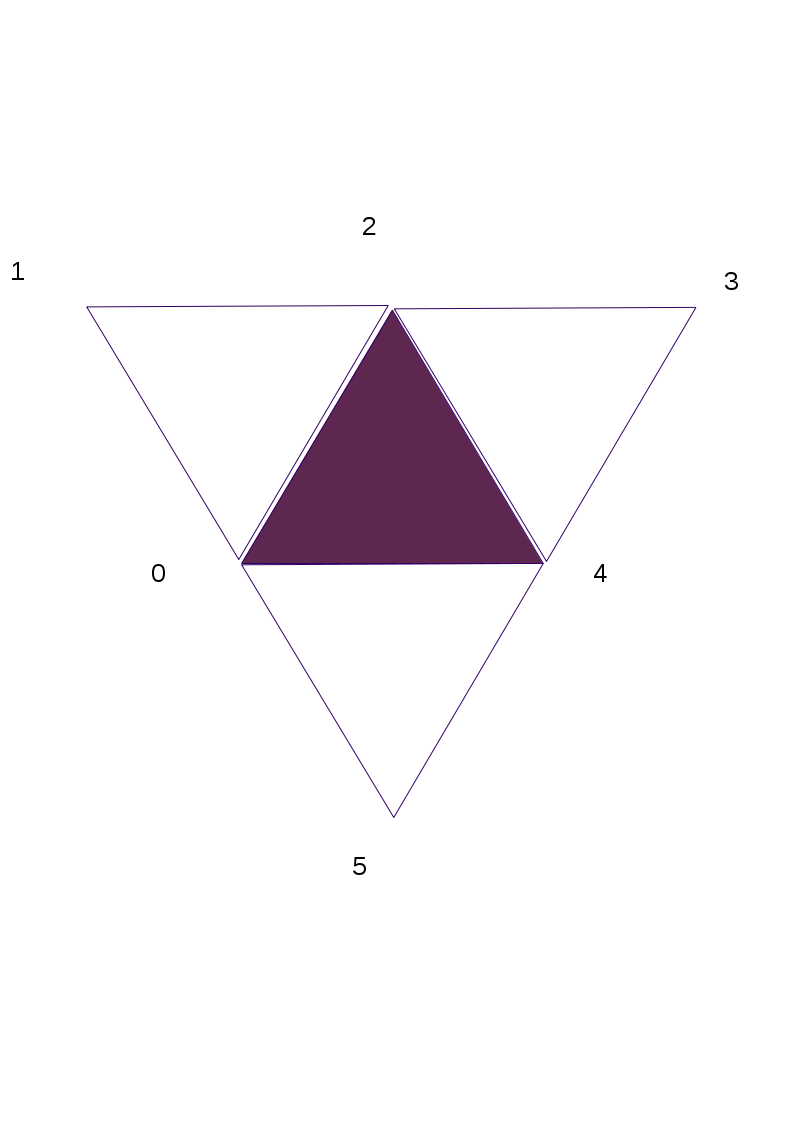
\includegraphics[width=10cm, trim = 0mm 50mm 0mm 50mm, clip]{triangle_adj.png}
\caption{The triangle with adjacency primitive. Indices 0, 2, 4 form the
original triangle and indices 1, 3, 5 are the adjacent vertices}
\end{figure}

To clarify what the object loader does, first we loop through every triangle in
the object mesh and create a hash table containing the neighbour information for
all of them. For the triangle (0,1,2) we begin by inserting the edge (0,1) and
the corresponding neighbour (2), then we insert the edge (1,2) and the
neighbour (0) and finally we insert the edge (2,0) and the neighbour (1). By
doing this for every triangle in the entire model mesh we can simply enter the
edges in any triangle and quickly recover the neighbours of each triangle, e.g.
if we input the edge (2,4) we look in our hash table and find the neighbour
(3). Finally we can construct our list of indices, used for drawing the object,
by looping through every vertex in every triangle and looking up the neighbours.

\subsection{Volumes}
To generate the actual shadow volumes in the geometry shader is actually rather straight forward. We begin by generating the front cap, we simply extract all triangles facing the light. If the dot product between the light direction and the triangle normal is positive the triangle faces the light (we take the light direction to point from the triangle towards the light source). The sides of the shadow volumes are found by taking each edge and checking whether both triangles sharing this edge faces the light or not, if one triangle faces the light but not the other then the edge is part of the side of the shadow volume. We create the sides of the shadow volumes by creating two triangles (one quad) covering the area between the edge and its projection at infinity. Projection at infinity is simple to achieve using homogeneous coordinates, simply put the w-coordinate to zero.

In this way we can effectively and simply generate the shadow volumes of our scene using the geometry shader.

\subsection{Geometry Shader syntax}
The geometry shader is a rather recent addition to the OpenGL pipeline and examples of how to use it are rather scarce. The few examples that do exist are usually written for older versions of OpenGL, where the geometry shader was an extension. Therefore, in most of the examples found online the syntax used is both dated and often also unusable in modern OpenGL usage. Something that caused quite a steep learning curve for using the geometry shader.

[VILL DU HA IN NÅT MER? JAG VET INTE ALLA PROBLEM DU HADE MED DET HÄR]

\section{Results}
Our implementation of shadow volumes is not entirely successful. We have never
been able to render correct shadows on any computer. As can be seen in [LÄMPLIG
FIGUR PÅ KANINER] we lack shadows on the lower rabbit, however the shadows on
the ground seem to have been rendered correctly. The shadow volumes also change
when the camera moves, something that they should definitely not do (unless
there is a light source attached to the camera), unless we run the program on
a computer in Southfork (which unfortunately has a stencil buffer of 0 bytes,
hardly useful for us) where the volumes do not change as the camera moves. The
volumes generated seem to be accurate, when rendered using the stencil buffer,
apart from changing as the camera moves around (again, except for when we use a
Southfork computer). If the camera is kept stationary and the light source
moved, the shadow volumes seem to behave correctly, something that implies that
the volumes computed with the geometry shader are indeed correct.

\section{Discussion}
As was mentioned above, our implementation of shadow volumes contain some bugs. We have been unable to find out what is causing this really strange behaviour and have no real ideas left. The error might be because of an error in the camera and or world matrices, however this seems unlikely as the scenes are normally rendered correctly, it might be that we multiply the vertices of the shadow volumes by the wrong combination of these matrices, but we have tried any combination of them and nothing has solved the problem. In order to really solve this problem we believe we would have to start over from scratch, simply redo the entire project and really focus on double checking every step of the generation of the shadow volumes. This seems like a rather extreme measure, but
we have tried every other possible solution and are currently at our wits' end.

\begin{thebibliography}{9}
\bibitem{gpug1}
	Randima Fernando,
	\emph{GPU Gems: Programming Techniques, Tips and Tricks for Real-Time
	Graphics}.
	Addison-Wesley Professional; First Edition edition, April 1, 2004.
	\url{http://http.developer.nvidia.com/GPUGems/gpugems\_copyrightpg.html}

\bibitem{CROW77}
  Franklin C. Crow,
  Shadow Algorithms for Computer Graphics.
  \emph{Computer Graphics, Vol 11, no.2}, pp242-7,1977.

\bibitem{HEIDMANN91}
  Tim Heidmann,
  Real Shadows Real Time.
  \emph{Iris Universe} 28, 28-31.
\bibitem{KOLIVAND13}
   H Kolivand, M Sunar,
   A Survey of Shadow Volume Algorithms in Computer Graphics.
   \emph{IETE TECHNICAL REVIEW.} 30, 1, 38-46, ISSN: 02564602
\bibitem{GEOM}
  OpenGL. Wiki,
  \emph{Geometry Shader},
  \url{https://www.opengl.org/wiki/Geometry_Shader}
\end{thebibliography}
\end{document}
